%\ctparttext{\color{black}\begin{center}
%		Esta es una descripción de la parte de informática.
%\end{center}}

%\part{Parte de informática}
\chapter{Introduction to Quantum Computing}

In this chapter we aim to provide a general overview ot the quantum computing fundamentals.

TODO: Add ref to Nielch. ; Cita necesaria para la compilación del latex: 
\cite{Smith1981}.

\section{The Quantum Bit}



\documentclass{article}
\usepackage[utf8]{inputenc}

\title{tfg cuantica}
\author{ocetebt }
\date{April 2021}

\documentclass{article}
\usepackage[utf8]{inputenc}

% TODO: quitar esto de aqui
\usepackage{graphicx}

\title{tfg cuantica}
\author{ocetebt }
\date{April 2021}

\begin{document}
	
	%\ctparttext{\color{black}\begin{center}
	%		Esta es una descripción de la parte de informática.
	%\end{center}}
	
	%\part{Parte de informática}
	%\chapter{Introduction to Quantum Computing}
	
	In this chapter we aim to provide a general overview to the quantum computing fundamentals required to understand. This development will be based on %TODO: añadir cita al Niel. La siguiente cita necesaria para la compilación del latex: 
	%\cite{Smith1981}.
	
	\section{Intuitive notions}
	
	\subsection{The Quantum Bit}
	
	The bit is the minimum measure of information on classical computation and classical information theory. Everything is this areas is built from scratch based on bits. Likewise, quantum computing and quantum information theory  are built upon the \textbf{qubit}. In this section we introduce the qubit and its basic properties.
	
	We will describe the qubit as a mathematical object, independent of its physical implementation. By describing them as mathematical entities we will be able to explore its properties mathematically without having to worry of the physics underneath. This let's us construct the quantum computing and quantum information theories without independent of the implementation. The physical realization of qubits will be described later on.
	
	So, what is a qubit? Just like the classical bit, a qubit has a state. For the bit, the two only possible states are either 0 or 1. A qubit can take the states $|0\rangle$ and $|1\rangle$ -corresponding to the classical states 0 and 1- or it can be in a \emph{linear combination} of them:
	
	$$ \psi = \alpha |0\rangle + \beta |1\rangle $$
	
	Where $\alpha$ and $\beta$ are complex numbers. This is often called \emph{superposition}. The $| \cdot \rangle$ is called the Dirac notation, usually used in quantum physics. So, although we will formalize them later on we can describe a qubit as a vector in a two-dimensional complex vector space, where $|0\rangle$ and $|1\rangle$ form an orthonormal basis called the \emph{computation basis}. $|0\rangle$ and $|1\rangle$ will be called \emph{computational basis states}.
	
	In classical computation, we may know the state of a bit by consulting it. That is, what can simply retrieve that information from the bit. The first difficulty we find in quantum computing is that once we \emph{measure} a qubit it \emph{collapses} to either $|0\rangle$ with probability $|\alpha|^2$, or to $|1\rangle$ with probability $|\beta|^2$. Thus, $|\alpha|^2 + |\beta|^2 = 1$. The measure obtained is gather after the qubit has collapsed to either one of this state, so the outcome may only be either $|0\rangle$ or $|1\rangle$.
	
	The superposition concept might be counter-intuitive, so let's look at them with an analogy. We can think of a coin being tossed as the following qubit:
	
	$$ \psi = \frac{1}{\sqrt{2}} |0\rangle + \frac{1}{\sqrt{2}} |1\rangle $$
	
	This does not represent a coin that has landed on its side, somehow fifty percent heads and fifty percent tails. It is a a spinning coin that has not landed yet. But upon measuring it, we make the coin land and see the result: either heads or tails and neither of the states in between. This example also describes the qubit collapse: once the coin has landed, we will see the same result every time we look at it -obviously-, just like every time a qubit is measured after the first measurement, the outcome will be the same since it has already collapsed. We will return to this state, which is usually denoted as $|+\rangle$.
	
	Given this behaviour, it is worth pointing out that we are not able to find $\alpha$ and $\beta$ by only measuring the qubit due to this collapsing behaviour. We can, however, initialize qubits in a certain state and alter its coefficients, thus knowing there exact value. However, once a single measurement is done, the qubit collapses and the $\alpha$ and $\beta$ values are "lost".
	
	At this point, the reader may ask themselves if a qubit may even physically exist, not just as a mathematical entity. Although we will study qubits mathematically and their physical implementations are discussed in Chapter [TODO: add chapter], we cannot proceed any further without providing a more accurate description of a qubit than a "coin being tossed".A possible realization of qubits are electrons in an single atom's orbit, as seen in Figure \ref{fig 1.1}. An electron in an orbit may be in the so-called ground and exited states, $|0\rangle$ and $|1\rangle$ respectively, depending on its energy. By 
	
	\begin{figure}[h]
		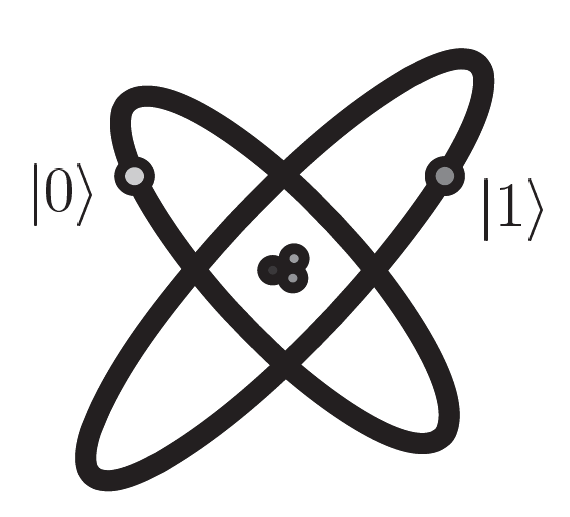
\includegraphics[scale=.5]{atom.png}
		\centering
		\caption{Qubit represented by two electron orbits in an atom, [TODO]}
		\label{fig 1.1}
	\end{figure}
	
	
	
\end{document}
